% new
\section{Reinforcement Learning}\label{chap2:reinforcement-learning}

Reinforcement learning is an umbrella term used to describe a class of algorithms for learning from experience. The basic idea is that a computer is given experiences in the real world (in a computer game, for example), and then has to learn how to act in that environment. The computer learns over time to increase its performance through trial and error and by watching what it does and making changes to its behavior policy. The performance is measured by the maximization of a reward function. Reinforcement learning is at the core of many of the most successful modern applications of artificial intelligence, such as AlphaGo, a computer that can play the board game Go better than any human being.

\begin{figure}[!ht]
    \centering
    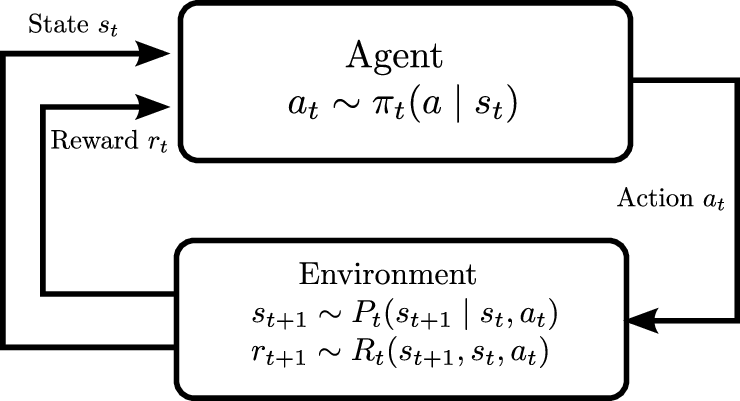
\includegraphics[width=0.50\textwidth]{images/agent-environment.png}
    \caption{Agent-environment relationship in an MDP according to \textcite{sutton1998introduction}: at each time step $t$, the agent observes the environment's current state $s_t$ and a reward signal $r_t$. The agent then selects an action $a_t$ given $s_t$ and following policy $\pi_t$. This action changes the environment state in the next time step to $s_{t+1}$ and yields reward $r_{t+1}$.
    }
    \label{fig:agent-environment}
\end{figure}


Despite the massive amount of recent research into the topic, reinforcement learning is still an extremely challenging field. This is due to the amount of information required to solve complex real world problems using reinforcement learning. For example, in the situation where one must create a simulation of a robot, one must take into account the factors and physics involved in the real world. 
% In fact, a recent paper on reinforcement learning concludes that, “The most common method for reinforcement learning involves learning the best policy in a simulated environment (or a set of them) through a brute force approach.”. 
% In fact, a recent paper on reinforcement learning concludes that, “The most common method for reinforcement learning involves learning the best policy in a simulated environment (or a set of them) through a brute force approach.”. 


Reinforcement learning is different from supervised learning in that the computer is given no labelled training data in the reinforcement learning case. Instead, it learns by trial and error and by watching its own actions. The idea is that, by observing what it does and seeing what results it gets, the computer will automatically learn what actions it should take to get better results in the future \cite{sutton2018reinforcement}.

% The subsections below describe 
Common concepts involved in a reinforcement learning problem are described below.

% Reinforcement learning is also referred to as a “model-free” learning algorithm. This is because the model that is learned, unlike in most other cases of machine learning, is not explicitly known beforehand


\textbf{Agent.}
The agent is the entity that actually does the learning. This is the actor that makes the decision for which action to take next based on the state observed from the environment \cite{sutton2018reinforcement}. For this action, the agent can receive a reward from the environment, from which the agent updates his value function or his policy. The agent then chooses a new action based on a new state and the interaction loop repeats. An complete interaction occurs at time step $t$, which is part of a sequence of time steps $t = 0, 1, ..., T$. 
The agent can be a single entity such as a robot or a group of entities that work together to solve the problem. The agent-environment interaction loop can be visualized in Figure \ref{fig:agent-environment}. 




\textbf{Action.}
The action refers to the action that is going to be taken. This could be one of the moves in a chess game, or it could be a move in a board game such as Go \cite{sutton2018reinforcement}.

\textbf{Learning from Experience.} The term “experience” as used in the context of reinforcement learning does not refer to a specific object or event. Rather, it refers to a sequence of events that have happened to the agent. However, the experiences that are fed into the reinforcement learning algorithm are derived directly from the environment \cite{sutton2018reinforcement}.

\textbf{Environment.}
The environment is the world in which the agent learns and collects observations of the state it finds itself in. It is also the world in which the agent must decide which actions to take. Accordingly, the environment provides rewards to the agent for each of these actions. Similarly, when the agent is, for example, damaged, the reward function decrements the reward that the agent receives for that action. The environment also provides the agent with feedback when it takes an action. It provides the agent with new visual observations, positions, velocity, health of enemy targets, etc. These observations are all factors that contribute to the agent’s perception of the environment. Environments, in general, can vary and be either a game of chess or a real-world application where one robot is being controlled by a human operator \cite{sutton2018reinforcement}.

A reinforcement learning environment can also be formally referred to as a Markov Decision Process (MDP) in other contexts, where each state is a possible outcome of the environment and each action is a possible change to the environment. 
An MDP is a formalism that can describe any decision-making process that can be described by a transition matrix. 
Moreover, for a reinforcement learning algorithm used in RL, an MDP may be thought of as a discrete-time Markov chain, where time is broken into discrete slots of a specified duration, and state is broken into discrete states.
This formalism allows a generalised analysis of the behaviour of an agent in terms of the utility or benefit of the agent in any state and any action taken in any state. It is described by a 5-tuple $(S,A,R,P,\mu)$, where:
\begin{itemize}
    \item $S$ is a set of states the environment can be in,
    \item $A$ is set of actions the agent can select,
    \item $R(s,a,s')$ is the reward function that maps state-action-next-state tuples to real valued rewards,
    \item $P(s'|s,a)$ is the probability of transitioning to state $s'$ given previous state $s$ and the agent choosing action $a$ while in $s$,
    \item $\mu(s)$ is the probability of starting in state $s$.
\end{itemize}
If an environment is fully observable, the agent has full knowledge of the state it is in. In a partially observable environment, the appropriate formalism is a Partially Observable Markov Decision Process (POMDP), where the agent must rely on its internal knowledge of its surroundings to make decisions. This is a generalization of the MDP to cases where the environment is partially observable, and it includes a set of observations $O$ and a conditional probability distribution, $P(o|s)$, for what observation is seen in which state \cite{sutton2018reinforcement}.


% There are two ways to make a policy in reinforcement learning. One way is to design a deterministic policy and then search through a set of possible actions (the policy). The other way is to search for an optimal policy, which is the solution to a dynamic programming equation. In both cases, there are two components that must be learned: the reward function and the value function. The reward function specifies the value of each action (change in state). The value

% The following figure illustrates the relationship between the environment and the agent, including the actions and observations that make up the state.

\textbf{Reward Signal and Return.}
A reward signal describes how well the agent did in a given situation. A reward signal can be thought of as a kind of scoreboard. It will assign a numerical score to each of the actions available to the agent in a given state. These scores are then combined to calculate a global reward which is to be maximized \cite{sutton2018reinforcement}.
In other words, the reward signal $R_t$ is the reward the agent obtains at time step $t$. The cumulative reward $G_t$ from this signal is the agent's objective. A simple return is defined as:
\begin{gather}
    G_t = R_{t+1} + R_{t+2} + ... + R_{t+T} = \sum_{k=0}^{T-t-1} R_{t+1+k} \label{eu_reward_signal}
\end{gather}
where T is the final time step. A return can also include a discount rate $\gamma$ that discourages future rewards, as shown in \ref{eu_discounted_reward}. A discount rate is used, for example, if the MDP is a continuous problem that never ends or to include uncertainty of future predictions \cite{sutton2018reinforcement}.

\begin{gather}
    G_{t,discounted} = \sum_{k=0}^{T-t-1} \gamma^k * R_{t+1+k}. \label{eu_discounted_reward}
\end{gather}

         Additionally, it is worth mentioning that a \textbf{sparse} reward signal refers to the lack of instantaneous rewards or penalties given to the agent per transition regardless of distance to the goal. In other words, it rewards the agent in states that are close to a goal. In contrast, a \textbf{dense} reward function rewards (or penalizes) the agent at most of the transitions it takes. This feedback can be counterproductive since the agent could have too many distractions at each timestep. This concept will prove useful in Chapter \ref{chap:discussion}.

\textbf{Value Function.}
Whereas the reward signal assigns a reward to the actions that are available to the agent at a given state, the value function specifies what is good in the long run. The value function calculates a value for a state, as the expected cumulative reward from the rewards in the future states, starting from that state. \cite{sutton2018reinforcement}
In other words, the state-value function, $V_{\tau}(s)$ is the expected future reward starting from state $s$ and following policy $\pi$. It can be written as


\begin{gather}
   V_{\pi}(s)=\mathbb{E}_{\pi}\left\{r_{t} \mid s_{t}=s\right\}=\mathbb{E}_{\pi}\left\{\left(\sum_{k=0}^{T-t-1} \gamma^{k} r_{t+1+k}\right) \mid s_{t}=s\right\} \label{eu_valuefunction}
\end{gather}
 
where $\gamma$ is the discount rate, $s_t$ is the state at time step $t$, $r_t$ is the reward at time step $t$, and $\mathbb{E}$ is the expected value \cite{eriksson2021deep}. 

Figure \ref{fig:gridworld} shows a grid-world environment where the agent must move from one cell to another to reach the goal. Given that there is a pit in which the agent can fall in. If the agent falls it is penalized through a negative reward. Hence, the state-value function for the cells around the pit is lower to represent that these are unwanted states.

\begin{figure}[!ht]
    \centering
    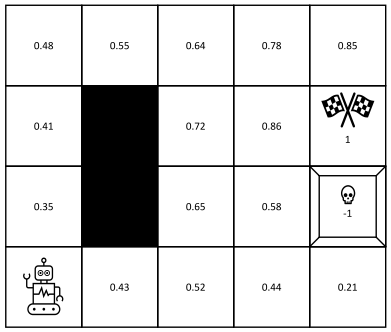
\includegraphics[width=0.55\textwidth]{images/gridworld.png}
    \caption{A grid-world environmentm. Each cell represents a state, and it is associated with a corresponding value, which is the value of the state-value function $V(s)$. The agent gets a reward when it reaches the goal with two flags, and given a penalty when it falls down the pit with a skull. Taken from \cite{eriksson2021deep}.
    }
    \label{fig:gridworld}
\end{figure}



\textbf{Policy.}
The policy $\pi$ is the rule by which the agent decides which actions to take. In other words, a policy is a mapping from states to actions, and it defines how the agent will behave at any given state \cite{sutton2018reinforcement}.
The policy, just like the reward function, is learned based on what the agent experiences, i.e., what states provide higher reward than others. A policy can be designed as a look-up table or through function approximation. When the policy is stochastic $\pi(a|s)$ denotes the probability to take action a given state s, and the optimal policy $\pi*$ is the policy that always prefers the action corresponding to the highest expected reward \cite{sutton2018reinforcement}. 

% To make a decision, the agent looks at the environment and then selects an action from a set of actions. If there are multiple actions to choose from, then the agent randomly selects one of them.

\textbf{Episode.}
An episode\textemdash also called a \textit{trajectory} or \textit{rollout}\textemdash is a single event (i.e., the sequence of steps of an agent) which is composed of several time steps. An episode is defined by a sequence of states and a set of actions in an MDP \cite{sutton2018reinforcement}. For example, a video game will have many states (positions of objects, etc.), and many actions (movements of the character). 
% In Figure X an episode is comprised of the states the agent traversed, to reach a terminal state, which is when the episode ends. 
% These interactions agent-environment . In this sense, an episode is really a game.
% An episode ends when the agent reaches a terminal state.
At the end of an episode, the environment is reset and a new episode begins with a fresh set of observations and actions.

\textbf{Exploration and Explotation.}
Reinforcement learning problems try to balance exploration of new states and explotation by following the actions to states that provide the best rewards. Finding an optimal policy requires the agent to explore new unknown states which could allow the discovery of a better state-value than the one currently known. 
%  It cannot just sit in one spot and follow a pre-determined action sequence. It has to explore the environment and get to know it so that it can then use that knowledge to make good choices in future situations.
An example of a policy that prefers exploration is the $\epsilon$-greedy policy. This policy assigns $\epsilon$ chance to choose a random action and $1-\epsilon$ to choose an action based on the known policy \cite{sutton2018reinforcement}.  


\subsection{Q-learning} \label{chap2:q-learning}
Q-learning one of the most well known reinforcement learning algorithms. It is a model-free learning algorithm and therefore it does not require any assumptions to be made about the environment or about the reward function.
At the start of each episode, the agent picks an action (also called a “policy”) from some policy distribution. The agent then receives a reward which is calculated based on the policy that was chosen. The agent then uses the reward to update the policy distribution, which is often called the Q-function. The Q-function is an action-value function $Q_\pi(s,a)$, which, in addition to the state-value function (reference), it also considers the action space \cite{sutton2018reinforcement}. It can be written as:

\begin{gather}
    Q_{\pi}(s, a)=\mathbb{E}_{\pi}\left\{r_{t} \mid s_{t}=s, a_{t}=a\right\}=\mathbb{E}_{\pi}\left\{\left(\sum_{k=0}^{T-t-1} \gamma^{k} r_{t+1+k}\right) \mid s_{t}=s, a_{t}=a\right\}
    
    \label{eu_q_learning}
\end{gather}

% Q-learning has proven to be a very successful and flexible algorithm, but it requires quite a bit of information to be provided in order to run efficiently.
Q-learning learns an optimal $\epsilon$-greedy policy. The agent has an $\epsilon$ chance of choosing a random action and $1-\epsilon$ of choosing an action based on the optimal policy. The optimal action is the one that maximizes the action-value function $\max _{a} Q_{\pi}(s, a)$ . 
% It algorithm starts
Q-learning works by starting from some arbitrary $Q_\pi(s,a)$, 
% state and action policy
and iteratively updates itself by taking into account the immediate rewards it receives. This is performed by taking an action and then updating its $Q_\pi(s,a)$ 
% policy distribution 
in the following manner:

\begin{gather}
   Q_{\pi}\left(S_{t}, A_{t}\right) \leftarrow Q_{\pi}\left(S_{t}, A_{t}\right)+\alpha\left[R_{t+1}+\gamma \max _{a} Q_{\pi}\left(S_{t+1}, a\right)-Q_{\pi}\left(S_{t}, A_{t}\right)\right]
   \label{eu_q_learning_policy}
\end{gather}

% $$\pi_{t+1}(s)=\frac{\pi_t(s)\cdot Q_\pi(s,a^*_t)}{\sum_{s'} \pi_t(s')\cdot Q_\pi(s',a^*_t)}$$

where $\lambda$ is the learning rate, $Q_\pi$ is the action-value function, and $\pi_t$ is the agent’s policy at step $t$. In the case of Q-learning, this is the optimal policy $\pi^*$. The learning rate determines how strongly the old values of $Q_\pi$ should be modified by the incoming update. This process is done until the episode ends. The environment then resets and the learning continues from a starting position \cite{sutton2018reinforcement}. The Q-learning algorithm can be seen in Algorithm \ref{alg:q-learning} below:

% \SetKwRepeat{Do}{do}{while}%


{\centering
\begin{minipage}{.8\linewidth}
    \begin{algorithm}[H]
      initialize $Q_\pi(s,a)$  with random values\;
      
      \For{each episode}{
        reset environment\;
    
          \While{\textbf{not} done}{
            choose action A based on state S using policy \pi\;
            
            perform action A and observe R,S'\;
            
            $Q_{\pi}(S, A) \leftarrow Q_{\pi}(S, A)+\alpha\left[R+\gamma \max _{a} Q_{\pi}\left(S^{\prime}, a\right)-Q_{\pi}(S, A)\right]$
            
            $S \leftarrow S^{\prime}$
            
            \If{episode end}{
                done\;
            }
          }
      }
      \caption{Q-learning}\label{alg:q-learning}
    \end{algorithm}
\end{minipage}
\par
}


After $n$ episodes, Q-learning should be able to learn a policy that allows the agent to solve the task successfully. There are several variants of Q-learning that differ from the method described above. A popular variant of Q-learning is SARSA (“Synchronous”, “Asynchronous”, “Reinforce”), which can be used for learning both discrete (e.g. chess, Go) and continuous (e.g. Atari games, robotics) problems \cite{sutton2018reinforcement}. Additionally, it is one of the algorithms available in the open source deep reinforcement learning OpenAI Gym \cite{openaigym}.

% https://deepsense.ai/what-is-reinforcement-learning-the-complete-guide/
% https://www.geeksforgeeks.org/what-is-reinforcement-learning/
% https://www.kdnuggets.com/2018/03/5-things-reinforcement-learning.html

% new

\subsection{Function Approximation}\label{chap2:function-approx}
Tables are a feasible solution for small state space searches for state-value and action-value functions. However, when the state space is large, such as in robotics applications, tables become impractical. 
Function approximation methods such as Gaussian processes, neural networks, and deep neural networks, make it easier to approximate large state-value and action-value functions \cite{sutton2018reinforcement}.
% were developed to work around this problem. 

% \textbf{Gaussian Processes.} 
% When a function  is continuous it can be approximated by a linear combination of Gaussian random variables. Let  be a Gaussian distribution with covariance function  such that  is a valid  for all  with probability. A Gaussian Process is a collection of  with  and  for any valid, and thus,  is a valid function approximator. The Gaussian process is useful for problems that are not known beforehand. The predictive distribution is given by

% where  is a multivariate Gaussian with mean  and covariance matrix  and  is a collection of  such that.

\subsubsection{Neural Networks.}
Neural networks are particularly good for modeling nonlinear relationships as they are essentially universal approximators.
They use a large number of interconnected neurons (perceptrons) to approximate the function $y = f*(x, \theta)$, which defines a mapping from input $x$ to output $y$, by learning the parameters $\theta$ \cite{eriksson2021deep}.

\begin{figure}[!ht]
    \centering
    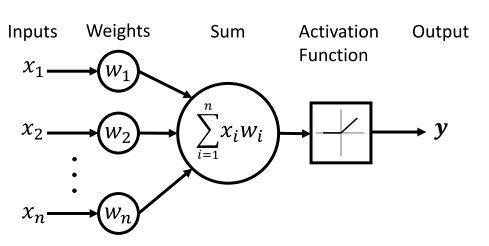
\includegraphics[width=0.5\textwidth]{images/neuron.png}
    \caption{Neuron. A single neuron consists of an input (or data) connection and an output (or hidden) connection. The input $x$ is multiplied by the training weights $\theta$ and summed. An activation function is then applied to the sum to obtain a nonlinear function $h(x,\theta)$ of the inputs.}
    \label{fig:neuron}
\end{figure}


    
A neuron consists of an input (or data) connection, and an output (or hidden) connection, as visualized in the model in Figure \ref{fig:neuron}. Inputs $x$ are multiplied by a set of training weights $\theta$ and summed. An activation function $h$ is then applied to the sum. The output $h(x,\theta)$ of a neuron is a nonlinear function of the input, and as a result a large number of neurons is needed to approximate a complex function. The weights are then trained by backpropagation in order to minimize the cost of the function approximation (i.e. the training set error). A common activation function, ReLU is defined as follows:
\begin{gather}
    h(x,\theta) =
    \begin{cases}
        0 & \text{if } z < 0,\\
        z & \text{if } z \ge 0,\\
    \end{cases}
    \label{eu_neural_network_cases}
\end{gather}
% then a neuron receives a set of inputs $v_i^j$ and returns an output $z_i^j$. The outputs are then combined with other outputs to form a neuron’s final output $o$.
% in continuous state space problems since they are relatively easy to train by back-propagation using a loss function.
where z is the summed output of the neuron. By tuning the weights of a neural network, non-linear functions can be approximated. Accordingly, a neural network could be leveraged to approximate the value function or policy of an agent by feeding state $s$ as input to the network \cite{eriksson2021deep}. 
% The weights of a neural network can be tuned through gradient descent.
A common and efficient method to tune the weights of a neural network is batch gradient descent. Gradient descent can be defined as
\begin{gather}
    \theta_{i, j} \leftarrow \theta_{i, j}-\alpha \frac{\partial L}{\partial \theta_{i, j}}
    \label{eu_neural_networks_weights}
\end{gather}
where $\alpha$ is the learning rate, $\theta_{i,j}$ are the neural network's weights and $L$ is the loss function.
A loss function is a measure of how well the neural network approximates the desired function. Common loss functions for value functions include squared error and mean squared error, where common loss functions for policy functions is cross-entropy. In the squared error $L=(y-\hat{y})^{2}$, $\hat{y}$ is the predicted output from the network and $y$ is the true value (ground truth).  For more information on backpropagation and gradient descent, see \cite{sutton2018reinforcement}. 

% Figure X: 
% Neuron with data input $x$ and hidden output $h$.

Neural networks have been shown to be a very powerful approach to nonlinear function approximation. For example, they are able to approximate the square root, logarithm, exponential, etc. However, this is not the case for complex functions, such as $f(x, \theta) = 1/1 + x \cdot \sin(\theta)$. While neural networks are an important tool in reinforcement learning, they are only good for low-dimensional functions and cannot be directly applied to high-dimensional or discrete state spaces. This has led to the emergence of methods using deep neural networks \cite{sutton2018reinforcement}.


% \textbf{Deep Neural Networks.}A deep neural network can be viewed as two neural networks or more, which are called hidden layers. The input data is the input layer and the predictions layer is the output layer. 
% The structure of a deep neural network is given by where and how layers interconnected. 
% Deep neural networks, as mentioned before, are trained by back-propagation

% Reinforcement learning is most successful when the value functions are approximated as neural networks, which is the focus of this work.

% In this case, it can be shown that the value function must satisfy the Bellman equation:
% Two popular function approximation methods are neural networks and Q-learning.
% https://www.baeldung.com/cs/ml-policy-reinforcement-learning#:~:text=A%20policy%20is%2C%20therefore%2C%20a,agent%27s%20state%20and%20the%20environment.
% https://towardsdatascience.com/policy-based-reinforcement-learning-the-easy-way-8de9a3356083

\subsubsection{Deep Neural Networks}
%  Accordingly, as the layers are stacked on top of each other, the number of parameters and amount of information needed to define the parameters increases. 

\begin{figure}[!ht]
    \centering
    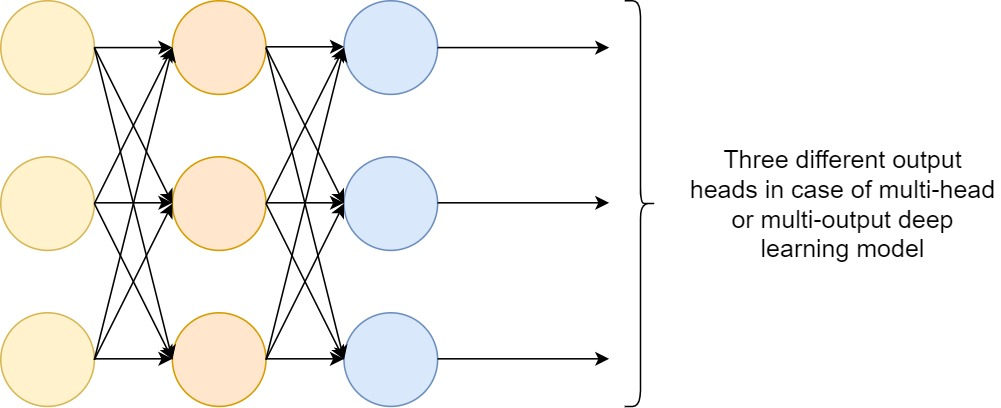
\includegraphics[width=0.7\textwidth]{images/multi_head_nn_exmp.jpg}
    \caption{Deep Neural Network with an input layer, a hidden layer and an multiple output heads. In actor-critic reinforcement learning problems and shared parameter networks, one head can be used as the prediction from the critic and another head as the prediction from the actor \cite{MultiHea51, sutton2018reinforcement}.
    }
    \label{fig:deep-nnetwork}
\end{figure}


Deep neural networks are a type of neural network which have been shown to work well for a variety of real world problems. In general, deep neural networks are a type of neural network that uses multiple layers of interconnected neurons, as shown in Figure \ref{fig:deep-nnetwork}. 
In situations when the input is an image, data manipulation strategies can be used, such as vectorization of the image so that it is compatible with the input a simple neural network expects. However, the loss of spatial information during the vectorization of the data (also called flattening) can be a problem if part of the solution requires to understand the relationship between the elements in a scene. Convolutional neural networks have therefore been shown to be a very effective solution to this problem since they are capable of processing images while keeping their matrix structure. These networks use a kernel of weights to "convolute" the image, which is also called "filter". A filter is applied over the entire input to output a new set of values. This process is repeated over all the different parts of the input and can be then fed to other types of network structures, such as fully connected layers \cite{eriksson2021deep}.
As of today, convolutional neural networks have proven to work well in many different domains, such as image classification, object detection, and semantic segmentation.


\subsection{Proximal Policy Optimization}\label{chap2:ppo}
Proximal Policy Optimization (PPO), designed by OpenAI, is a reinforcement learning algorithm that is known for performing better than one of the most popular reinforcement learning algorithms: DQN (also known as the Deep Q Network algorithm; which has roots in the theory presented in Section \ref{chap2:q-learning}).
PPO overcomes a lot of challenges that other methods struggle with such as sample efficiency, overall performance, and ease of implementation and tuning capabilities \cite{schulman2017proximal}. %16, 17 
Moreover, while algorithms like DQN learn from offline memory, PPO can do online learning without using a replay buffer for past experiences. In other words, it allows the agent to learn directly from the environment and discard the batch of experiences after a gradient update. 
Finally, PPO belongs to methods that leverage the state value function to update the policy. Actor-critic methods, as an extension of Q-learning, approximate the value function (critic) to assist in the policy (actor) updates.

The following subsections further introduce the fundamental concepts behind PPO, such as policy gradient and clipping, and the algorithm itself.


% Reinforcement Learning Algorithms

% Actor-Critic

% The actor-critic algorithm is an offshoot of PPO and is a more efficient variant of PPO. The algorithm uses both a

\subsubsection{Policy Gradient}
Policy Gradient methods estimate the optimal parametrized action policy $\pi(a \mid s, \theta)$ (i.e. which action is taken in each state) and are typically used in large state spaces. These methods learn the policy's parameter vector $\theta$ by learning the weights of a neural network. 
The parametrized policy $\pi(a \mid s, \theta)$ describes a distribution which gives a probability of choosing action $a$ given state $s$ and parameters $\theta$ at timestep $t$ as
\begin{gather}
    \pi(a \mid s, \theta)=\operatorname{Pr}\left\{A_{t}=a \mid S_{t}=s, \theta_{t}=\theta\right\}.
    \label{eu_policy_gradient}
\end{gather}
These methods aim to maximize the expected return $J(\theta)$, known also as the objective function or loss, by following the parametrized policy \cite{sutton2018reinforcement}. Gradient descent (or ascent) is then used to update the weights of the network as
\begin{gather}
   \theta_{t+1}=\theta_{t}+\alpha \widehat{\nabla J\left(\theta_{t}\right)}
   \label{eu_policy_gradient_update_weiights}
\end{gather}
where $\widehat{\nabla J\left(\theta_{t}\right)}$ is an estimate of the gradient of the objective function (expected return) \cite{3}. A standard gradient estimator for these methods is
\begin{gather}
    \widehat{\nabla J\left(\theta_{t}\right)}=\hat{E}_{t}\left[\nabla_{\theta} \log \pi_{\theta}\left(a_{t} \mid s_{t}\right) \hat{A}_{t}\right]
    \label{eu_policy_gradient_estimator}
\end{gather}
where $\pi_{\theta}$ is the parametrized stochastic policy, $\hat{E}_{t}$ is the expectation across a batch of experiences and $\hat{A}_{t}$ is an estimator of the advantage function at timestep t \cite{sutton2018reinforcement}. 
The respective objective function for the policy gradient estimator is therefore
\begin{gather}
  L^{\mathrm{PG}}(\theta)=\widehat{J(\theta)}=\hat{E}_{t}\left[\log \pi_{\theta}\left(a_{t} \mid s_{t}\right) \hat{A}_{t}\right].
  \label{eu_policy_gradient_obj_function}
\end{gather}
Optimizing on $L^{P G}$ is, however, not justified, given that it leads to destructively large policy updates \cite{schulman2017proximal}.

\subsubsection{Clipping}
PPO builds upon the concepts mentioned above and simplifies the concepts introduced by TRPO by proposing a clipped "surrogate" objective and retaining parallel performance. 

\begin{figure}[!ht]
    \centering
    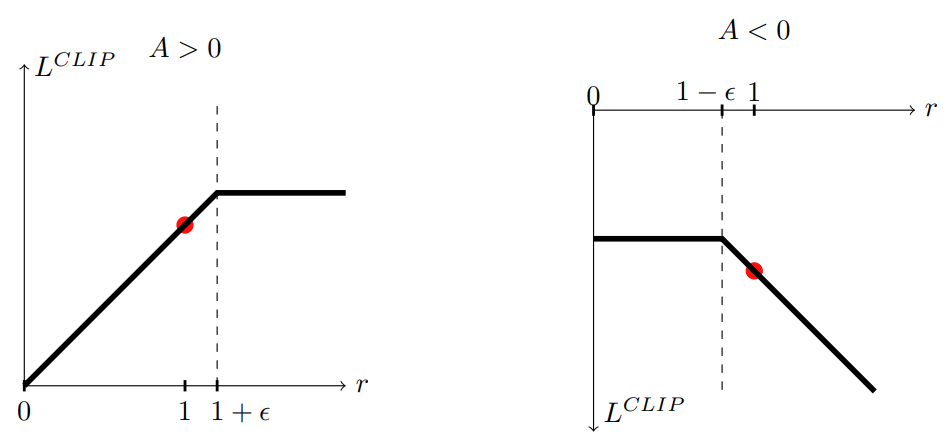
\includegraphics[width=0.7\textwidth]{images/LCLIP_PPO.png}
    \caption{Plots showing one term (i.e., a single timestep) of the surrogate function L CLIP as a function of the probability ratio r, for positive advantages (left) and negative advantages (right). The red circle on each plot shows the starting point for the optimization, i.e., r = 1. Note that L CLIP sums many of these terms.
    \cite{schulman2017proximal}.
    }
    \label{fig:LCLIP}
\end{figure}

First, the probability ratio between the policy with the current parameters and the policy with the old parameters is defined as
\begin{gather}
    r(\theta)=\frac{\pi_{\theta}(a \mid s)}{\pi_{\theta_{\text {old }}}(a \mid s)}.
    \label{eu_policy_gradient_probability_ratio}
    
\end{gather}
Then, the objective function of TRPO (on policy) is:
\begin{gather}
  L^{\mathrm{TRPO}}(\theta)=\mathbb{E}\left[r(\theta) \hat{A}_{\theta_{\text {old }}}(s, a)\right].
  \label{eu_ppo_policy_trpo_objective_function}
\end{gather}
However, given that the ratio between the policies can grow to be very large, PPO constraints the ratio $r(\theta)$ to stay in a small interval around $1$ through the introduction of an additional hyperparameter $\epsilon$ \cite{schulman2017proximal}. The value function loss then becomes
\begin{gather}
    L^{\mathrm{CLIP}}(\theta)=\mathbb{E}\left[\min \left(r(\theta) \hat{A}_{\theta_{\mathrm{old}}}(s, a), \operatorname{clip}(r(\theta), 1-\epsilon, 1+\epsilon) \hat{A}_{\theta_{\mathrm{old}}}(s, a)\right)\right]
    \label{eu_ppo_value_function}
\end{gather}
where the function $\operatorname{clip}(r(\theta), 1-\epsilon, 1+\epsilon)$ constraints the ratio to a maximum and a minimum. Subsequently, the objective function of PPO takes a pessimistic lower bound to the loss by keeping the minimmum of the unclipped $r(\theta) \hat{A}_{\theta_{\text {old }}}(s, a)$ and the clipped ratio times the advantage estimator \cite{schulman2017proximal}. The advantage estimator is defined by
\begin{gather}
  \hat{A}_{t}=\delta_{t}+(\gamma \lambda) \delta_{t+1}+\ldots+(\gamma \lambda)^{T-t+1} \delta_{T-1}
  \label{eu_ppo_advantage_estimator}
\end{gather}
where
\begin{gather}
  \delta_{t}=r_{t}+\gamma V(s_{t+1})-V(s_{t})
  \label{eu_ppo_smoothing_coeff}
\end{gather}
and $\lambda$ is a smoothing coefficient. 
  
% \subsubsection{Policy Iteration}
% Policy Iteration is a model-based algorithm for reinforcement learning. Unlike the model-free Q-learning algorithm, it assumes a model of the environment. The agent can then perform actions and the agent’s behavior can be calculated by performing an appropriate simulation of the environment. When it receives the environment’s observation, the agent can determine whether it believes the environment is in a certain state or not. The agent then performs actions and the environment responds. This process is repeated multiple times and the agent’s reward is calculated. The reward can then be used to update the environment model. The process of learning from experience can be summarized by the following algorithm.

\subsubsection{Algorithm}
% A common practice to reduce the variance of the gradient of the expected return estimates is to add a baseline function $b(st)$ inside the expectation. Typical choices are the average reward $\bar{R}$, or the state value function $V(s)$. For more information on baseline functions, refer to \cite{}.
Most techniques for calculating variance-reduced advantage-function estimators leverage a learned state-value function V(s) as baseline function and PPO is no different \cite{schulman2017proximal}. If using a neural network architecture that shares parameters between the two predictions heads for the policy and value functions, PPO proposes to add a value function error term to the policy surrogate and an entropy term to encourage sufficeint exploration. This new loss is defined as
\begin{gather}
    L_{t}^{C L I P+V F+S}(\theta)=\hat{\mathbb{E}}_{t}\left[L_{t}^{C L I P}(\theta)-c_{1} L_{t}^{V F}(\theta)+c_{2} S\left[\pi_{\theta}\right]\left(s_{t}\right)\right]
\end{gather}
where $c1$,$c2$ are coefficients, $S$ denotes the entropy bonus and $L_{t}^{V F}$ is the value function loss \cite{schulman2017proximal}. In other words, $L_{t}^{C L I P}(\theta)$ is the loss for the actor network and $L_{t}^{V F}$ is the loss for the critic network. The loss of the value function used in PPO is defined as
\begin{gather}
    L^{\mathrm{VF}}=\left(V_{\theta}\left(s_{t}\right)-V_{t}^{\text {target }}\right)^{2}
\end{gather}
where $V_{\theta}\left(s_{t}\right)$ is also known as the critic return and in some implementations is seen as $\delta_{t} + V_{\theta}\left(s_{t}\right)$. Similarly, the term $S_{\pi_{\theta}}\left(s_{t}\right)$ is an entropy bonus that promotes exploration \cite{schulman2017proximal}. Concretely, this is the Shannon entropy and is computed by
\begin{gather}
    S_{\pi_{\theta}}\left(s_{t}\right)=-\sum_{i=1}^{n} \pi_{\theta}\left(a_{i} \mid s_{t}\right) \log \left(\pi_{\theta}\left(a_{i} \mid s_{t}\right)\right.
\end{gather}
In summary, the main idea of PPO is to avoid large policy updates during training by clipping the ratio between the old and the current policy. It successfully combines function approximation with policy optimization while showing great performance \cite{schulman2017proximal}. Finally, the algorithm is described in Algorithm \ref{alg:ppo} below:

{\centering
\begin{minipage}{.8\linewidth}
    \begin{algorithm}[H]
        initialize $\theta$\;
      
        \For{iteration i=0,1,...}{
            \For{time step t=0,1,..., T}{
                sample time step with policy $\pi_{\theta, \text { old }}$\;
                calculate advantage $\hat{A}_{t}$\;
            }
            \For{epoch k=0,1,..., K}{
                optimize $L^{\mathrm{CLIP}+\mathrm{VF}+\mathrm{S}}$ with respect to $\theta$\;
                update $\theta$\;
            }
        }
      \caption{PPO}\label{alg:ppo}
    \end{algorithm}
\end{minipage}
\par
}



%  The environment includes a simulation of the voxels, such that voxel positions have a value (e.g. their distance to a goal voxel) which changes based on actions in the environment. Voxel positions also have an octree node in which they are embedded. This allows the voxels to have a 3D spatial location in the environment. The voxels are also assigned a classification (e.g. “rock”, “fertilizer”, “air”, etc.). The voxels also receive a reward which is related to the classification they represent

%  We formulate the reinforcement learning problem as one of minimizing a loss function defined on exploration and goal selection. Specifically, the exploration policy is a probability distribution that selects the voxel from the voxel pool to observe based on their classification. The goal is a set of octree nodes, which are a tree in which each node has an octree parent node and a set of child nodes that are octree children nodes of the parent node. For each goal node, there is an associated reward value.


% In the simplest scenario, the goal is always the goal node. We propose two different models of goal selection. The first model is a fully deterministic approach where a goal node is randomly selected from the goal set. The goal nodes are randomly ordered before being selected from the goal set, and the order of nodes can be randomized. The second model is a semi-deterministic approach where a goal node is selected based on a probability distribution from a goal distribution. The goal distribution is defined by a Gaussian kernel function which is used to select nodes from a set of nodes in a specific region of the environment.

% deterministic
% semi-deterministic



% method (old)
% based on actions in the environment. Voxel positions also have an octree node in which they are embedded. This allows the voxels to have a 3D spatial location in the environment. The voxels are also assigned a classification (e.g. “rock”, “fertilizer”, “air”, etc.). The voxels also receive a reward which is related to the classification they represent.

% we train the agent with a genetic algorithm [@mouret]



% method, solid
% Reinforcement learning is an umbrella term used to describe a class of algorithms for learning from experience. The basic idea is that a computer is given experiences in the real world (in a computer game, for example), and then has to learn how to act in that environment. The computer learns over time to increase its performance through trial and error and by watching what it does and making changes to its behavior policy. In our context, reinforcement learning means learning how to generate exploration policies given intrinsic rewards based on voxels and octree nodes in an unknown environment.

% The environment includes a simulation of the voxels, where every voxel has been generated through a voxel generating algorithm that traversed the original mesh of each object. Moreover, each voxel has a position and a pose (e.g. near the mesh of the object it belongs to) which remains set until the end of an episode. An episode can end when the agent hits a wall or all the voxels have been scanned. Once an episode ends, domain randomization allows to change the locations and poses of the objects of interest, to promote the generalized exploration of unknown environments.


% Our agent can therefore learn how to behave in the voxel-based environment, while also embedding the positions it traverses and the positions of the scanned voxels in the nodes of an octree. This motivates the agent to explore new nodes in the environment, both with and without voxels. The voxels are therefore not assigned any classification (e.g. "rock, "fertilizier", "bike", etc.). Instead, they are concrete 3D representations of the objects of interest to the agent, which serve as intrinsic rewards to the agent. Ideally, the voxels would provide a different reward related to the classification they represent, but the semantic to each object has been determined out of scope to focus rather in a general exploration of the environment.

% another wording
% The problem of reinforcement learning is therefore a multi-agent interaction problem. In our case, a single agent is in charge of the whole process and tries to maximize its cumulative reward over time. The agent interacts with the environment and learns from its experience by choosing actions that maximize its rewards. As it is more likely that it is more beneficial for the agent to explore than to stay within a known area, the environment rewards the agent for exploration. To promote generalization, we allow the agent to explore the environment in an incremental manner: the environment randomly changes the positions of the objects of interest in the simulation, and the agent is not

% In order to demonstrate AEIL, I will take the case of a computer simulation where the goal of the robot is to traverse a maze. While this is a trivial task in the real world, for the sake of the experiment, the maze is a simulation of the real world. The maze is divided into an x-axis and a y-axis, with all obstacles located at one of the endpoints. As with real life, the maze is generated randomly, and the computer learns as it moves forward. In this case, the computer starts from the top left corner of the maze, and the goal is to find a way